\documentclass[aspectratio=169]{beamer}

% ─── Theme & Colors ───────────────────────────────────────────────────────────
\usetheme{Madrid}
\usecolortheme{owl}   % dark background
\setbeamertemplate{navigation symbols}{}
\setbeamertemplate{footline}[frame number]

\definecolor{accent}{RGB}{0,188,212}        % cyan accent
\definecolor{bg}{RGB}{18,18,28}             % deep navy background
\definecolor{surface}{RGB}{30,30,46}        % card background
\definecolor{textlight}{RGB}{220,220,235}   % light text
\definecolor{muted}{RGB}{140,140,165}       % muted text

\setbeamercolor{normal text}{fg=textlight,bg=bg}
\setbeamercolor{structure}{fg=accent}
\setbeamercolor{frametitle}{fg=accent,bg=surface}
\setbeamercolor{title}{fg=white}
\setbeamercolor{subtitle}{fg=accent}
\setbeamercolor{author}{fg=muted}
\setbeamercolor{date}{fg=muted}
\setbeamercolor{institute}{fg=muted}
\setbeamercolor{block title}{fg=white,bg=accent!80!black}
\setbeamercolor{block body}{fg=textlight,bg=surface}
\setbeamercolor{itemize item}{fg=accent}
\setbeamercolor{itemize subitem}{fg=accent!60}
\setbeamercolor{enumerate item}{fg=accent}
\setbeamercolor{alerted text}{fg=accent}
\setbeamercolor{palette primary}{bg=surface,fg=accent}
\setbeamercolor{palette secondary}{bg=surface,fg=accent}
\setbeamercolor{palette tertiary}{bg=accent,fg=white}

\setbeamertemplate{frametitle}{%
  \vskip2pt
  \insertframetitle
  \vskip-2pt
  \textcolor{accent}{\rule{\textwidth}{0.4pt}}
  \vskip2pt
}

% ─── Packages ─────────────────────────────────────────────────────────────────
\usepackage[utf8]{inputenc}
\usepackage{graphicx}
\usepackage{subcaption}
\usepackage{amsmath}
\usepackage{tikz}
\usepackage{xcolor}
\usepackage{booktabs}

% Helper: colored box
\newcommand{\filterbox}[2]{%
  \begin{block}{#1}
    #2
  \end{block}%
}

% ─── Meta ─────────────────────────────────────────────────────────────────────
\title{\textbf{Image Filter Application}}
\subtitle{ZPOe 25/26 — Applied Image Processing in C++/OpenCV}
\author{Adar Otieno \quad Deniz Aksoy \quad Eyobed Awel Nuri}
\institute{Brno University of Technology \\ Faculty of Information Technology}
\date{\today}

% ─── Document ─────────────────────────────────────────────────────────────────
\begin{document}

% ── Title Slide ──
\begin{frame}[plain]
  \begin{tikzpicture}[remember picture, overlay]
    \fill[bg] (current page.south west) rectangle (current page.north east);
    \fill[accent!20!bg] (current page.south west) rectangle +(\paperwidth, 0.5pt);
    \fill[accent] (current page.south west) rectangle +(\paperwidth, 0.25pt);
  \end{tikzpicture}
  \vfill
  \centering
  {\color{muted}\small Brno University of Technology — FIT}\\[0.4cm]
  {\color{white}\LARGE\textbf{Image Filter Application}}\\[0.3cm]
  {\color{accent}\large ZPOe 25/26 — Applied Image Processing in C++/OpenCV}\\[0.6cm]
  \textcolor{muted}{\rule{0.5\textwidth}{0.4pt}}\\[0.5cm]
  {\color{textlight}
    Adar Otieno \textbullet\ Deniz Aksoy \textbullet\ Eyobed Awel Nuri}\\[0.2cm]
  {\color{muted}\small\today}
  \vfill
\end{frame}

% ── Outline ──
\begin{frame}{Outline}
  \tableofcontents
\end{frame}

% =============================================================================
\section{Project Overview}
% =============================================================================

\begin{frame}{Project Overview}
  \begin{columns}[T]
    \column{0.5\textwidth}
      \begin{block}{Goal}
        Design and implement \textbf{12 image processing filters} applied to human face images. Filters are built manually using pixel-level C++ code — no high-level OpenCV abstractions.
      \end{block}
      \vspace{0.4cm}
      \begin{block}{Tech Stack}
        \begin{itemize}
          \item \textbf{Language:} C++17
          \item \textbf{Library:} OpenCV (HighGUI, core)
          \item \textbf{Build:} CMake
        \end{itemize}
      \end{block}
    \column{0.45\textwidth}
      \begin{block}{Contribution Split}
        \begin{itemize}
          \item 4 filters per student
          \item Shared interactive GUI
          \item Unified \texttt{Filter} struct interface
        \end{itemize}
      \end{block}
      \vspace{0.4cm}
      \begin{block}{Architecture}
        Each filter is registered as a function pointer inside a \texttt{Filter} struct carrying author, name, description, and the \texttt{apply()} callback.
      \end{block}
  \end{columns}
\end{frame}

% ── Application ──
\begin{frame}{Interactive Application}
  \begin{columns}[T]
    \column{0.55\textwidth}
      \begin{itemize}
        \item Built on \textbf{OpenCV HighGUI}
        \item \textbf{Two trackbars:}
        \begin{itemize}
          \item Image selector (iterates \texttt{data/} directory)
          \item Filter selector (12 entries)
        \end{itemize}
        \item Side-by-side 800×600 preview window
        \item Dynamic metadata panel (filter name, author, description)
      \end{itemize}
      \vspace{0.4cm}
      \begin{alertblock}{Running}
        \texttt{mkdir build \&\& cd build}\\
        \texttt{cmake .. \&\& make}\\
        \texttt{./project}
      \end{alertblock}
    \column{0.4\textwidth}
      \begin{block}{Filter Interface}
        \small
        \texttt{struct Filter \{}\\
        \quad\texttt{string author;}\\
        \quad\texttt{string name;}\\
        \quad\texttt{string description;}\\
        \quad\texttt{Mat (*apply)(const Mat\&);}\\
        \texttt{\};}
      \end{block}
  \end{columns}
\end{frame}

% ── Input Images ──
\begin{frame}{Input Images}
  \centering
  \textcolor{muted}{Four face images used as the common test dataset}\\[0.3cm]
  \begin{columns}
    \column{0.23\textwidth}\centering
      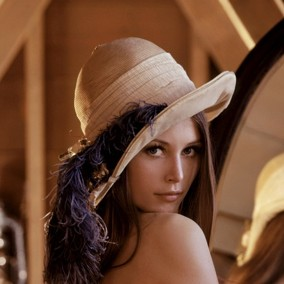
\includegraphics[width=\linewidth]{../report/assets/original_0.png}
    \column{0.23\textwidth}\centering
      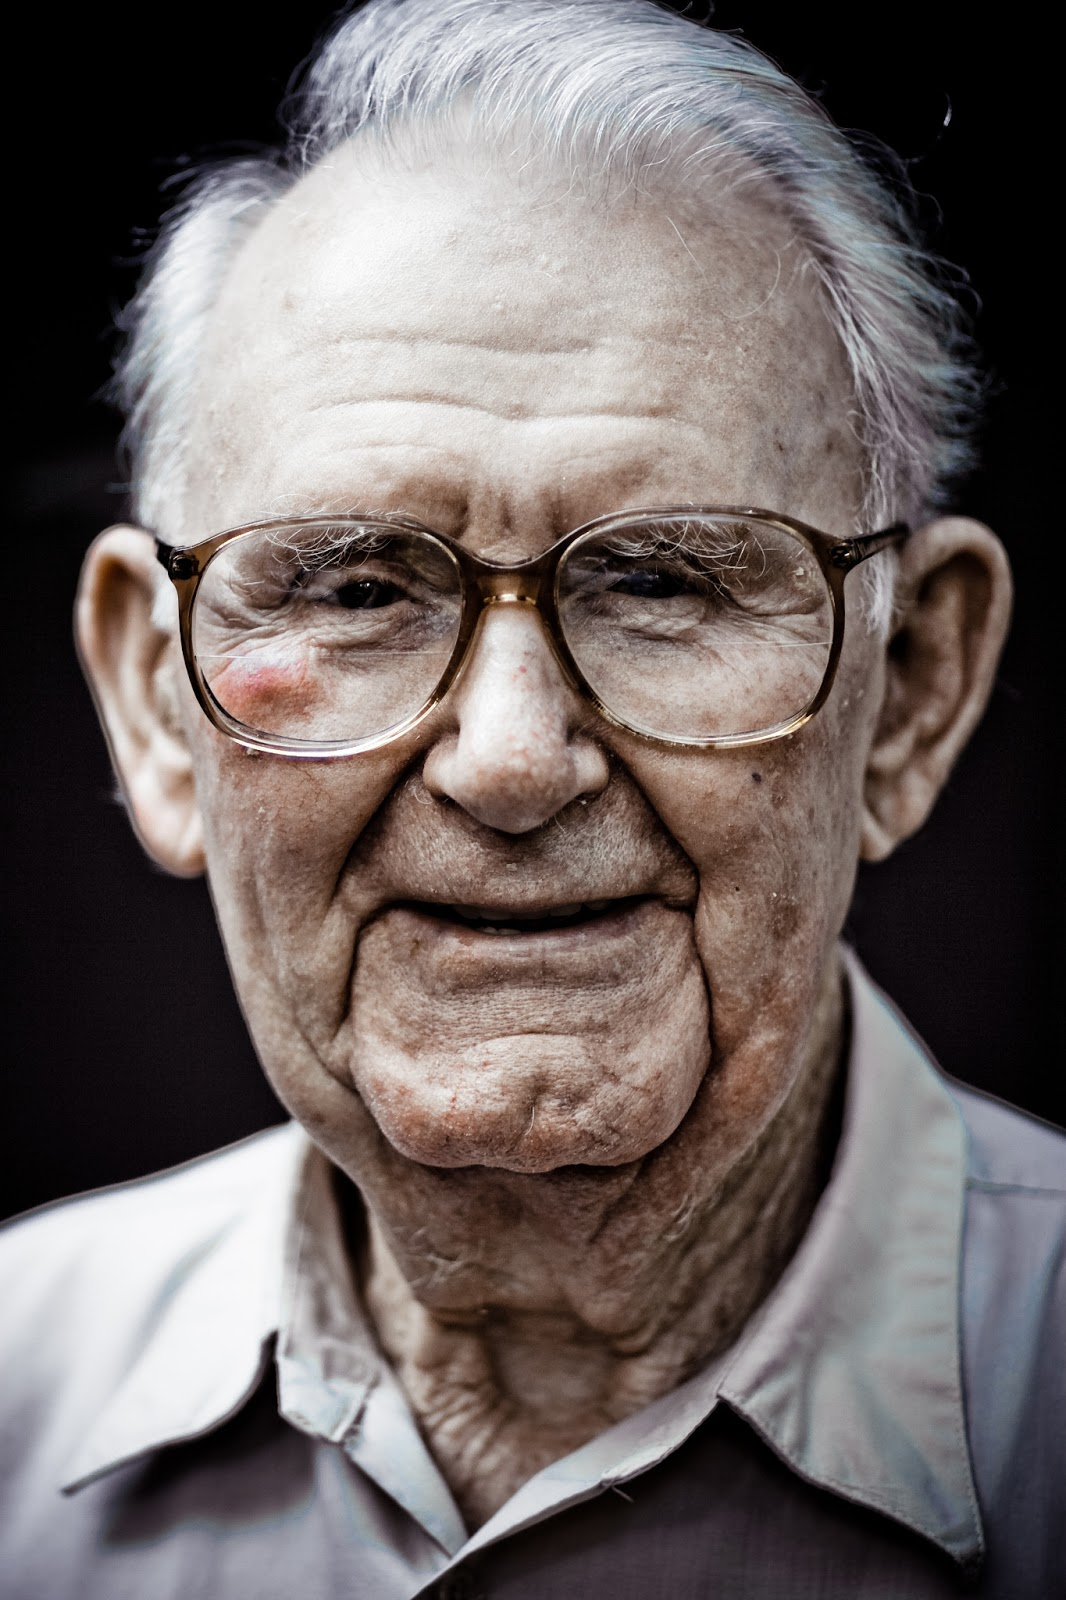
\includegraphics[width=\linewidth]{../report/assets/original_1.png}
    \column{0.23\textwidth}\centering
      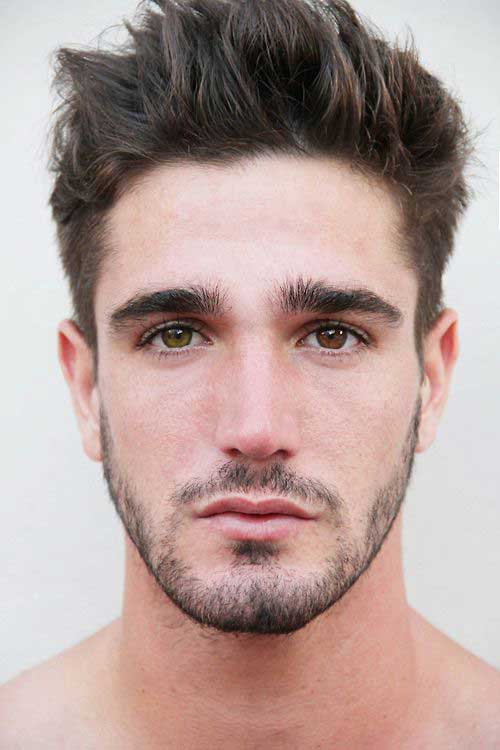
\includegraphics[width=\linewidth]{../report/assets/original_2.png}
    \column{0.23\textwidth}\centering
      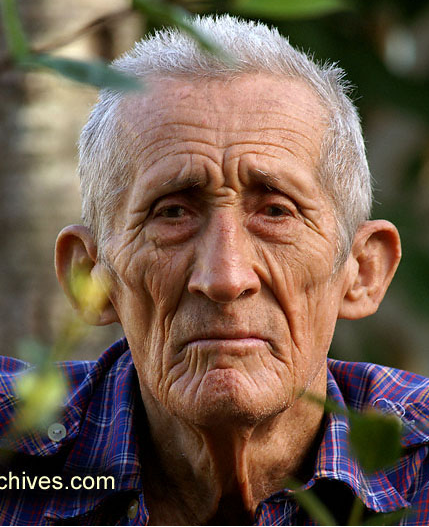
\includegraphics[width=\linewidth]{../report/assets/original_3.png}
  \end{columns}
\end{frame}

% =============================================================================
\section{Eyobed's Filters}
% =============================================================================

\begin{frame}{Eyobed's Filters — Overview}
  \begin{columns}[T]
    \column{0.48\textwidth}
      \filterbox{[Hist Eq] Histogram Equalization}{
        Redistributes luminance values via a CDF remap in YCrCb space. Boosts contrast without color shift.
      }
      \vspace{0.3cm}
      \filterbox{[Lens] Lens Distortion}{
        Inverse geometric mapping with radial coefficient $k$. Simulates barrel distortion.
      }
    \column{0.48\textwidth}
      \filterbox{[Post] Posterize}{
        Quantizes each BGR channel into $L=8$ levels using a precomputed LUT. $O(W \times H)$.
      }
      \vspace{0.3cm}
      \filterbox{[Vig] Vignette Blur}{
        15×15 box blur blended with original via a radial distance mask $d \in [0,1]$.
      }
  \end{columns}
\end{frame}

\begin{frame}{Histogram Equalization}
  \begin{columns}[T]
    \column{0.45\textwidth}
      \textbf{Algorithm:}
      \begin{enumerate}
        \item Convert BGR $\to$ YCrCb
        \item Compute PDF: $\displaystyle PDF(i) = \frac{\text{count}(i)}{W \cdot H}$
        \item Compute CDF: $\displaystyle CDF(i) = \sum_{j=0}^{i} PDF(j)$
        \item Remap: $\text{Out}(x,y) = \text{round}(CDF \times 255)$
        \item Convert YCrCb $\to$ BGR
      \end{enumerate}
      \vspace{0.3cm}
      \textcolor{muted}{Complexity: $O(W \times H)$}
    \column{0.5\textwidth}
      \centering
      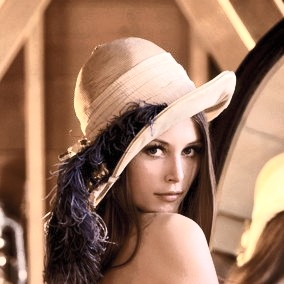
\includegraphics[width=0.48\linewidth]{../report/assets/histogram_eq_filtered_0.png}\hfill
      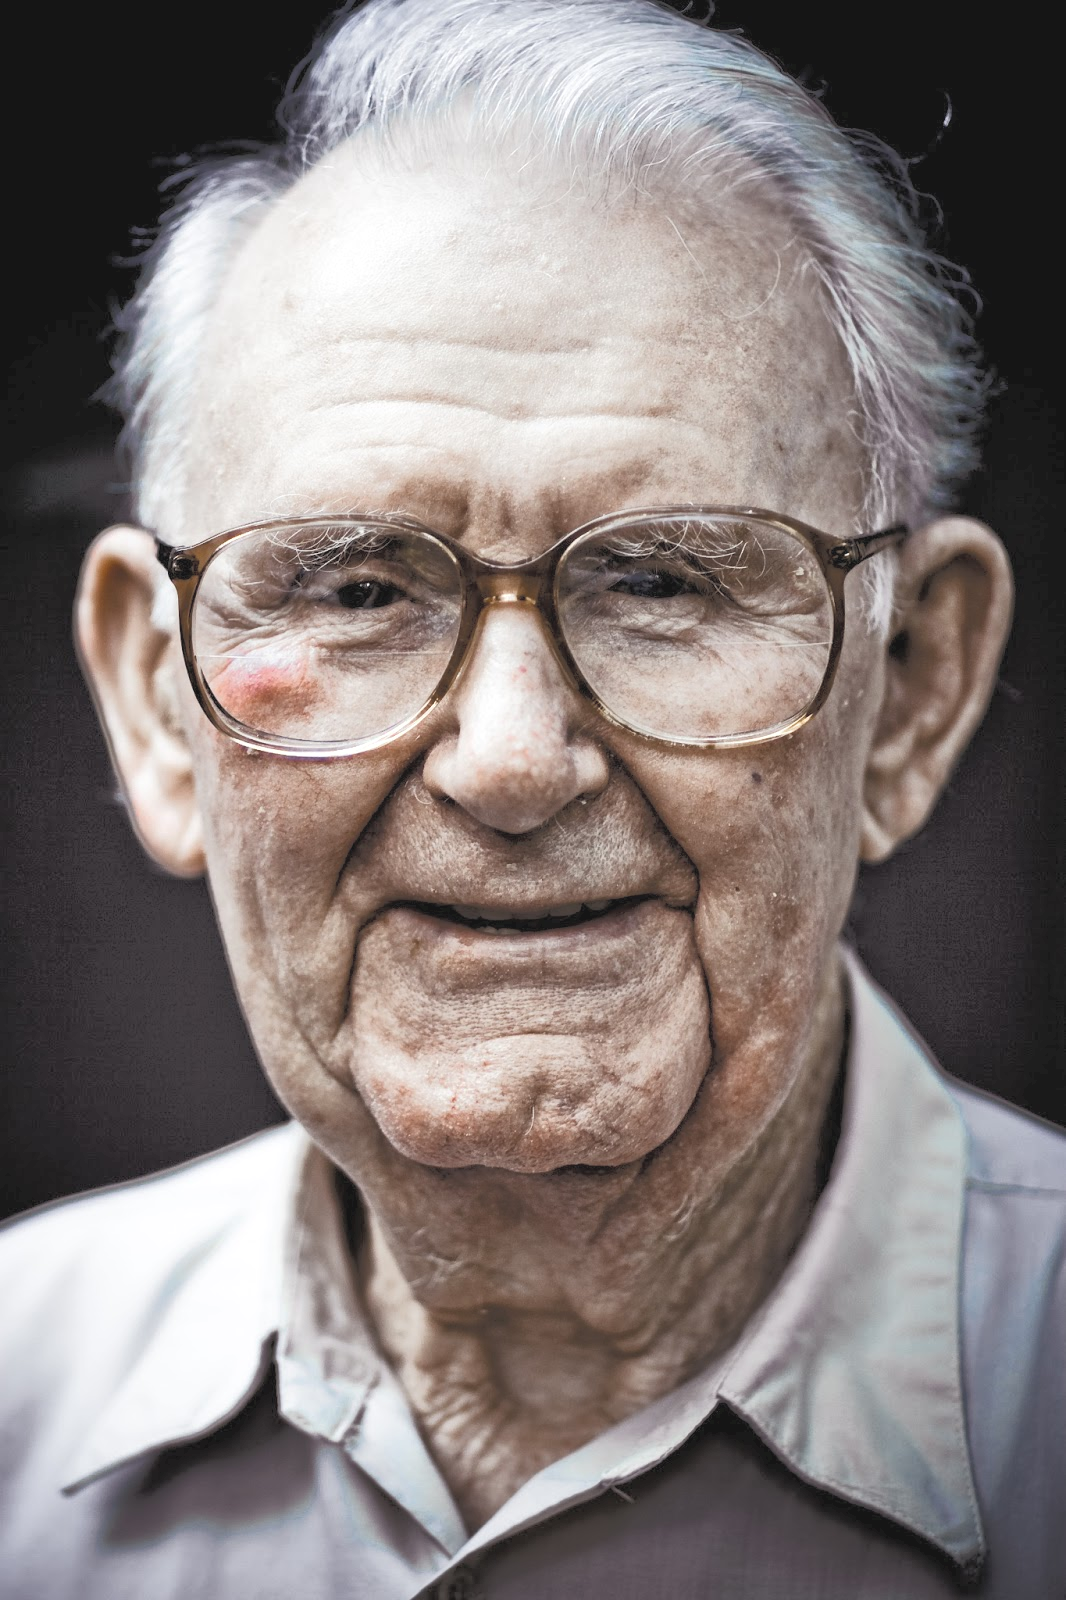
\includegraphics[width=0.48\linewidth]{../report/assets/histogram_eq_filtered_1.png}\\[2pt]
      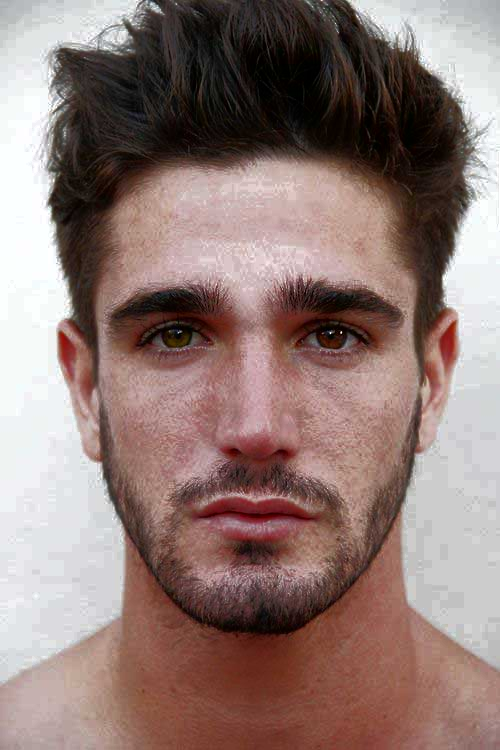
\includegraphics[width=0.48\linewidth]{../report/assets/histogram_eq_filtered_2.png}\hfill
      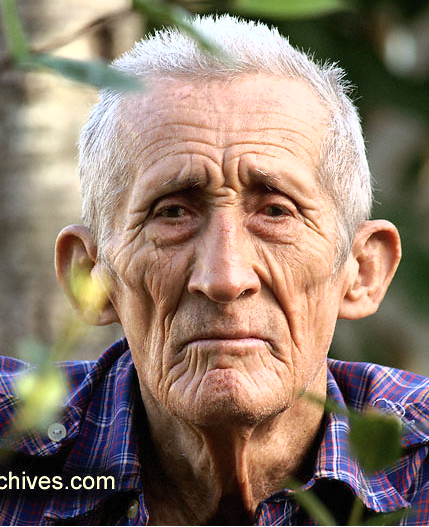
\includegraphics[width=0.48\linewidth]{../report/assets/histogram_eq_filtered_3.png}
  \end{columns}
\end{frame}

\begin{frame}{Lens Distortion}
  \begin{columns}[T]
    \column{0.45\textwidth}
      \textbf{Inverse Geometric Mapping:}
      \begin{enumerate}
        \item Normalize: $d_x = \frac{x-c_x}{R},\; d_y = \frac{y-c_y}{R}$
        \item Distort: $\text{dist} = 1 + k(d_x^2+d_y^2)$\\
              Positive $k$ → barrel distortion
        \item Map back: $s_x = d_x \cdot \text{dist} \cdot R + c_x$
      \end{enumerate}
      \vspace{0.3cm}
      \textcolor{muted}{Nearest-neighbor interpolation. $O(W \times H)$.}
    \column{0.5\textwidth}
      \centering
      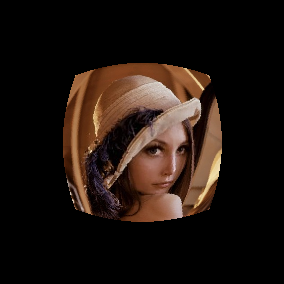
\includegraphics[width=0.48\linewidth]{../report/assets/lens_distortion_filtered_0.png}\hfill
      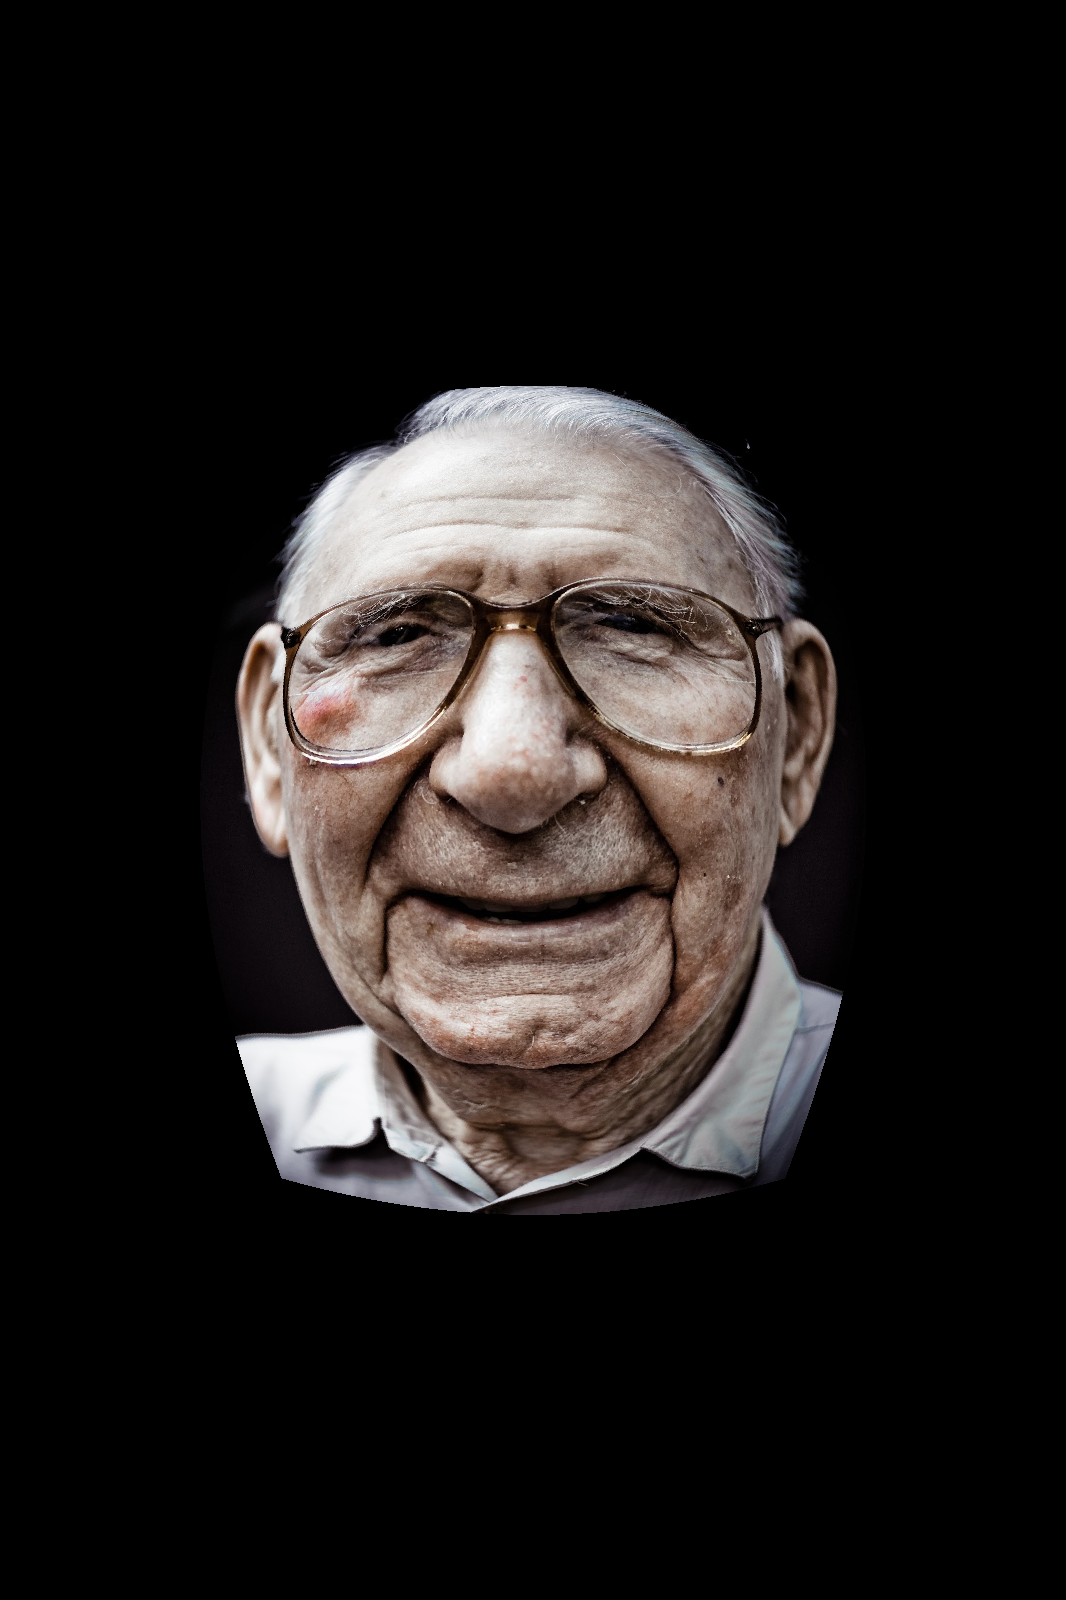
\includegraphics[width=0.48\linewidth]{../report/assets/lens_distortion_filtered_1.png}\\[2pt]
      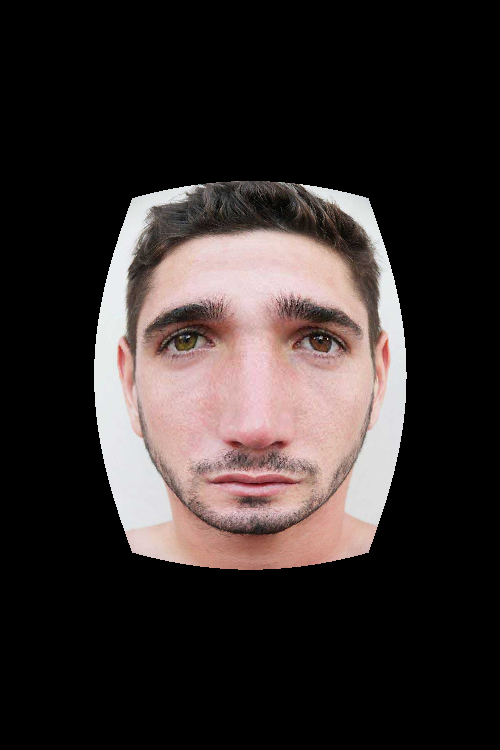
\includegraphics[width=0.48\linewidth]{../report/assets/lens_distortion_filtered_2.png}\hfill
      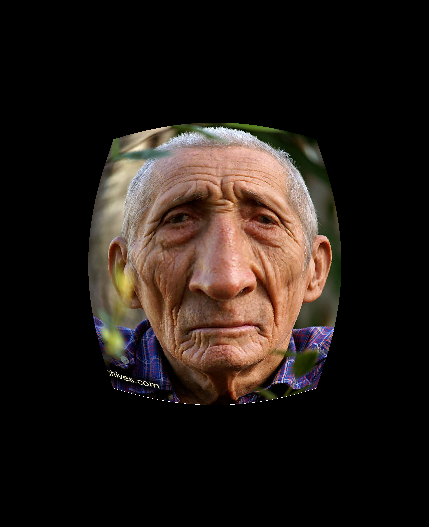
\includegraphics[width=0.48\linewidth]{../report/assets/lens_distortion_filtered_3.png}
  \end{columns}
\end{frame}

\begin{frame}{Posterize}
  \begin{columns}[T]
    \column{0.45\textwidth}
      \textbf{LUT-based Quantization ($L=8$):}
      \begin{enumerate}
        \item Step: $\displaystyle\text{step} = \frac{255}{L-1} \approx 36.4$
        \item Build LUT: $\text{level}_i = \text{round}(i / \text{step})$\\
              $\text{LUT}[i] = \text{round}(\text{level}_i \times \text{step})$
        \item Apply: $\text{Out}_c(x,y) = \text{LUT}[\text{In}_c(x,y)]$
      \end{enumerate}
      \vspace{0.3cm}
      \textcolor{muted}{$O(W \times H)$ + $O(256)$ for LUT.}
    \column{0.5\textwidth}
      \centering
      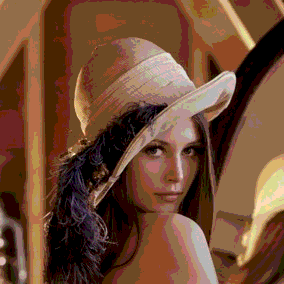
\includegraphics[width=0.48\linewidth]{../report/assets/posterize_filtered_0.png}\hfill
      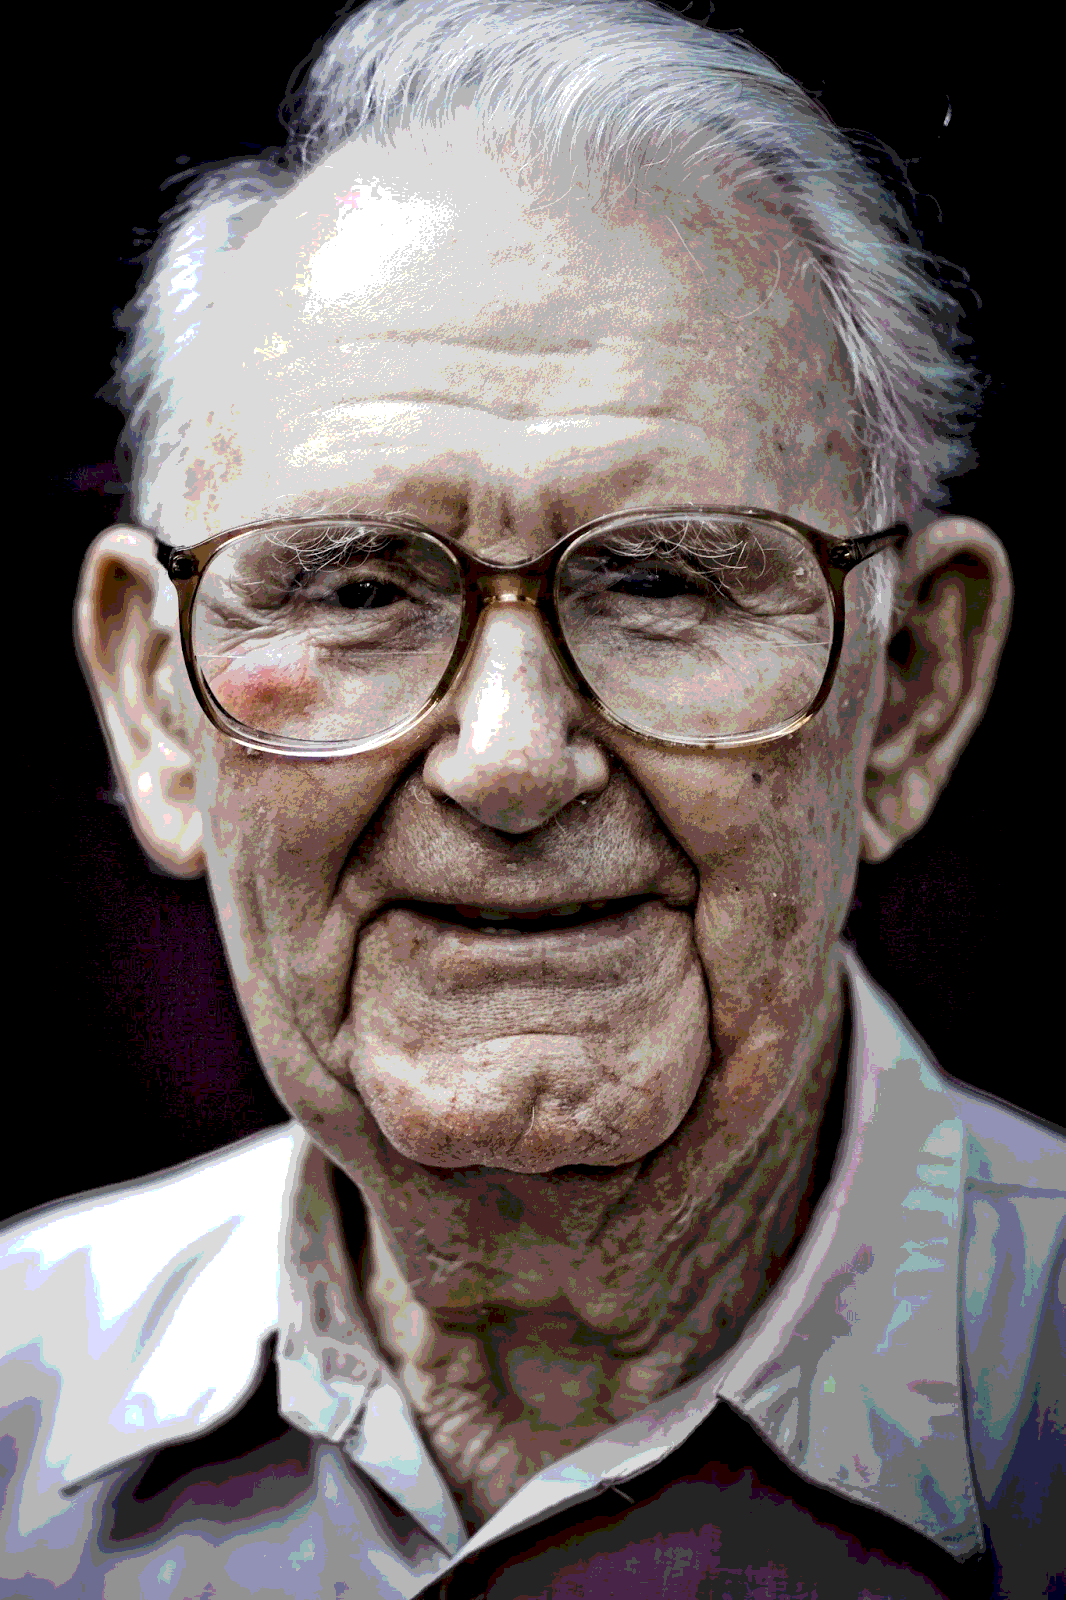
\includegraphics[width=0.48\linewidth]{../report/assets/posterize_filtered_1.png}\\[2pt]
      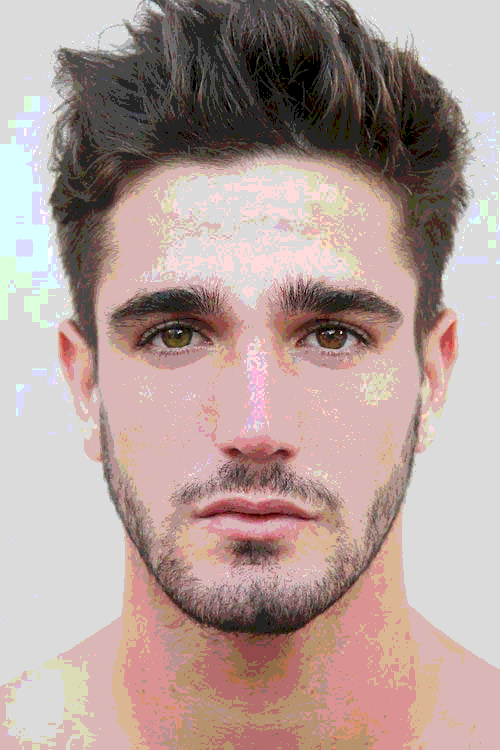
\includegraphics[width=0.48\linewidth]{../report/assets/posterize_filtered_2.png}\hfill
      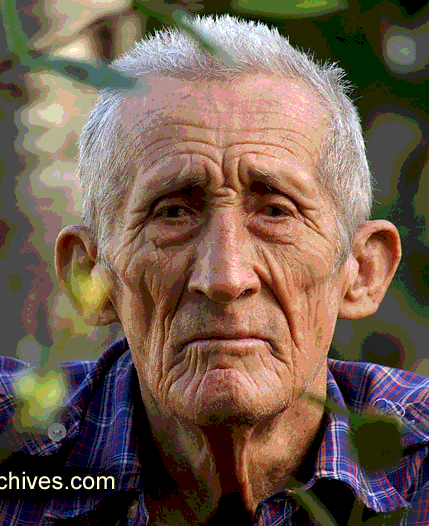
\includegraphics[width=0.48\linewidth]{../report/assets/posterize_filtered_3.png}
  \end{columns}
\end{frame}

\begin{frame}{Vignette Blur}
  \begin{columns}[T]
    \column{0.45\textwidth}
      \textbf{Two-Stage Radial Blend:}
      \begin{enumerate}
        \item Box blur (15×15 kernel):\\
              $\text{Blur} = \frac{1}{225}\!\sum_{dy,dx=-7}^{7}\!\text{In}(x{+}dx, y{+}dy)$
        \item Radial mask:\\ $d = \frac{\sqrt{(x-c_x)^2+(y-c_y)^2}}{R}$
        \item Blend:\\ $\text{Out} = \text{In}(1-d) + \text{Blur} \cdot d$
      \end{enumerate}
      \vspace{0.3cm}
      \textcolor{muted}{Single pass. $O(W \times H)$.}
    \column{0.5\textwidth}
      \centering
      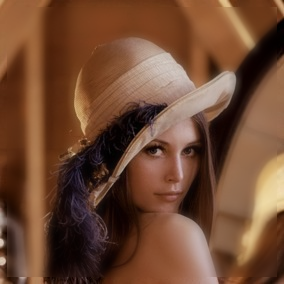
\includegraphics[width=0.48\linewidth]{../report/assets/vignette_blur_filtered_0.png}\hfill
      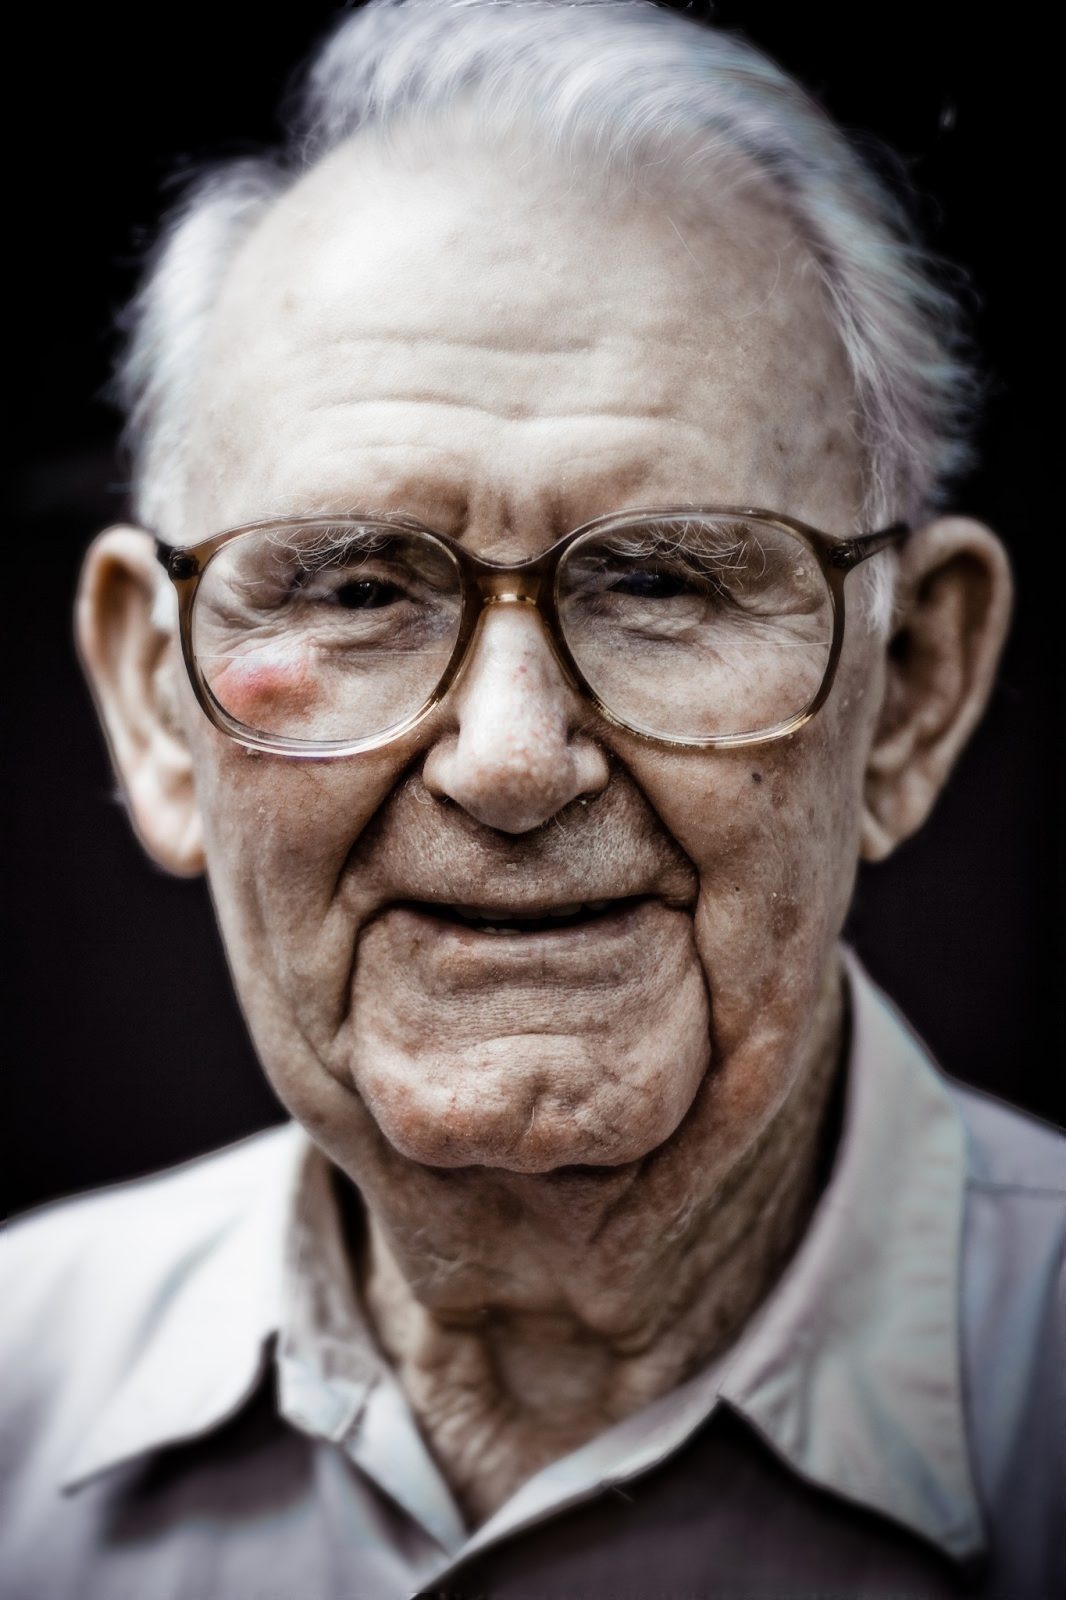
\includegraphics[width=0.48\linewidth]{../report/assets/vignette_blur_filtered_1.png}\\[2pt]
      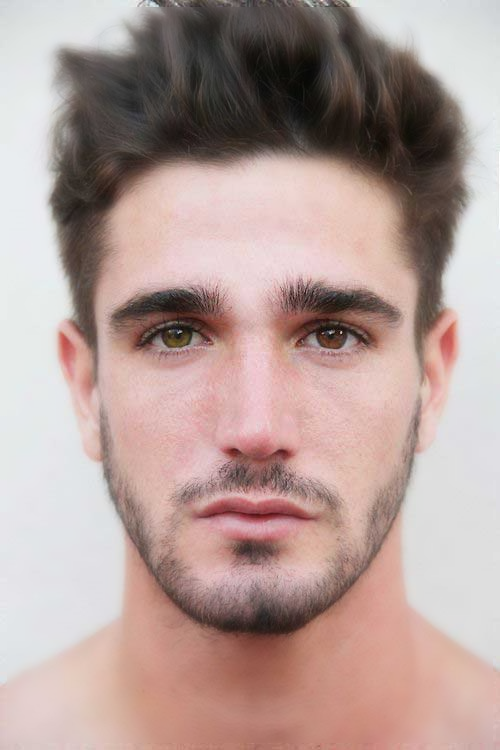
\includegraphics[width=0.48\linewidth]{../report/assets/vignette_blur_filtered_2.png}\hfill
      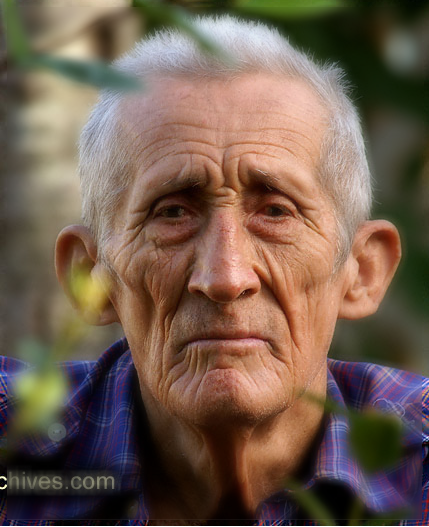
\includegraphics[width=0.48\linewidth]{../report/assets/vignette_blur_filtered_3.png}
  \end{columns}
\end{frame}

% =============================================================================
\section{Adar's Filters}
% =============================================================================

\begin{frame}{Adar's Filters}
  \begin{columns}[T]
    \column{0.48\textwidth}
      \filterbox{[Emboss] Relief Emboss}{
        Computes the difference between top-left and bottom-right neighbors, offset by 128 to produce a 3D gray-relief texture.
      }
      \vspace{0.3cm}
      \filterbox{[Dodge] Dodge}{
        Applies the Color Dodge formula per channel:\\
        $\text{Out} = \frac{p \times 255}{\max(1,\; 255-p)}$\\
        Blows out highlights, raises contrast sharply.
      }
    \column{0.48\textwidth}
      \filterbox{[Swirl] Swirl}{
        Polar-coordinate warp: each pixel's radius drives a nonlinear angular rotation before being mapped back.
      }
      \vspace{0.3cm}
      \filterbox{[Bloom] Bloom}{
        Extracts pixels above intensity 180, applies a 7×7 brute-force blur, and additively composites the glow onto the original.
      }
  \end{columns}
\end{frame}

% =============================================================================
\section{Deniz's Filters}
% =============================================================================

\begin{frame}{Deniz's Filters — Overview}
  \begin{columns}[T]
    \column{0.48\textwidth}
      \filterbox{[Threshold] Threshold}{
        Luminance $L = 0.299R + 0.587G + 0.114B$. Pixels above threshold $T$ → white; otherwise black.
      }
      \vspace{0.3cm}
      \filterbox{[Diffuse] Diffuse}{
        Frosted-glass effect: each pixel is replaced by a randomly sampled neighbor within a fixed radius.
      }
    \column{0.48\textwidth}
      \filterbox{[Crosshatch] Crosshatch}{
        Procedural sketch rendering using repeating mathematical line patterns to simulate pencil hatching.
      }
      \vspace{0.3cm}
      \filterbox{[Hue] Hue Rotate}{
        HSV-space hue shift: $H' = (H + \Delta H) \bmod 180$.\\
        $\Delta H = 60°$ preserves geometry and brightness.
      }
  \end{columns}
\end{frame}

\begin{frame}{Threshold \& Diffuse Results}
  \begin{columns}
    \column{0.48\textwidth}
      \centering
      \textbf{Threshold}\\[4pt]
      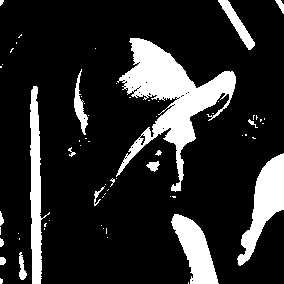
\includegraphics[width=0.48\linewidth]{../report/assets/threshold_1.png}\hfill
      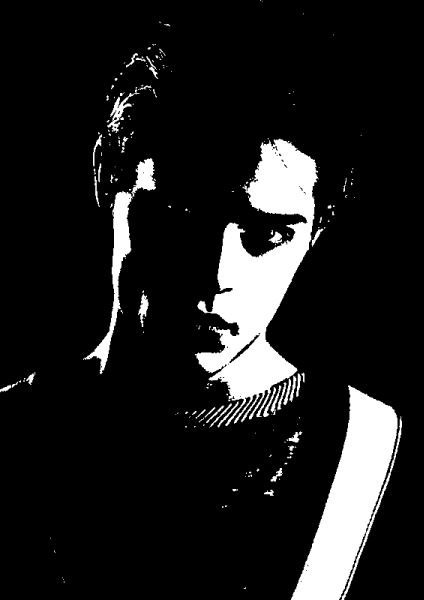
\includegraphics[width=0.48\linewidth]{../report/assets/threshold_2.png}\\[2pt]
      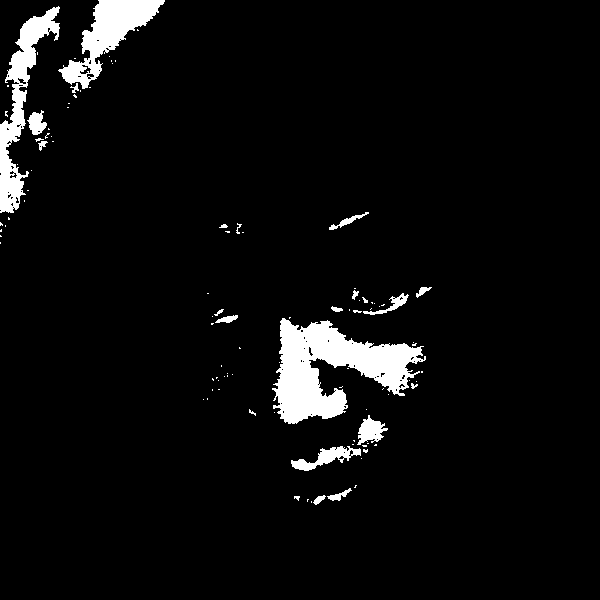
\includegraphics[width=0.48\linewidth]{../report/assets/threshold_3.png}\hfill
      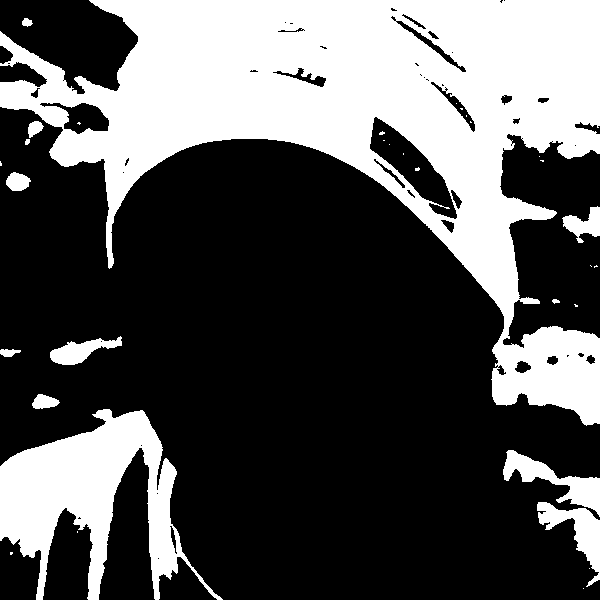
\includegraphics[width=0.48\linewidth]{../report/assets/threshold_4.png}
    \column{0.48\textwidth}
      \centering
      \textbf{Diffuse}\\[4pt]
      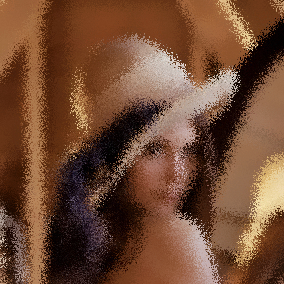
\includegraphics[width=0.48\linewidth]{../report/assets/diffuse_1.png}\hfill
      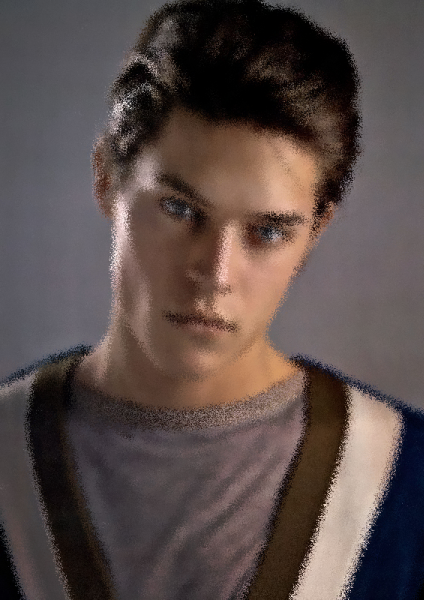
\includegraphics[width=0.48\linewidth]{../report/assets/diffuse_2.png}\\[2pt]
      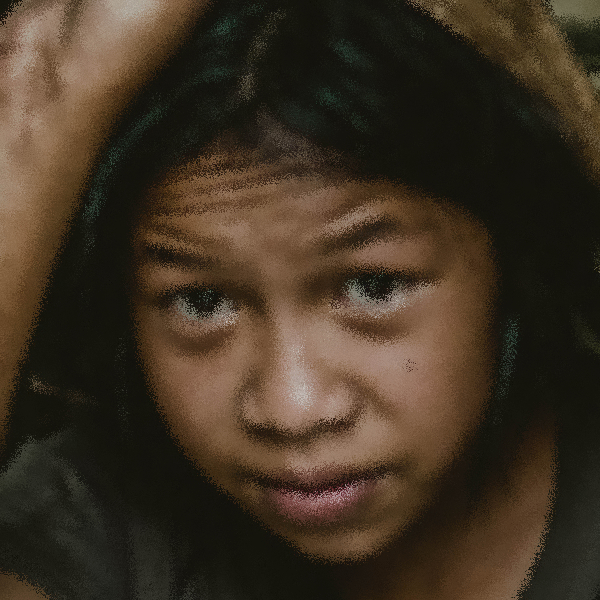
\includegraphics[width=0.48\linewidth]{../report/assets/diffuse_3.png}\hfill
      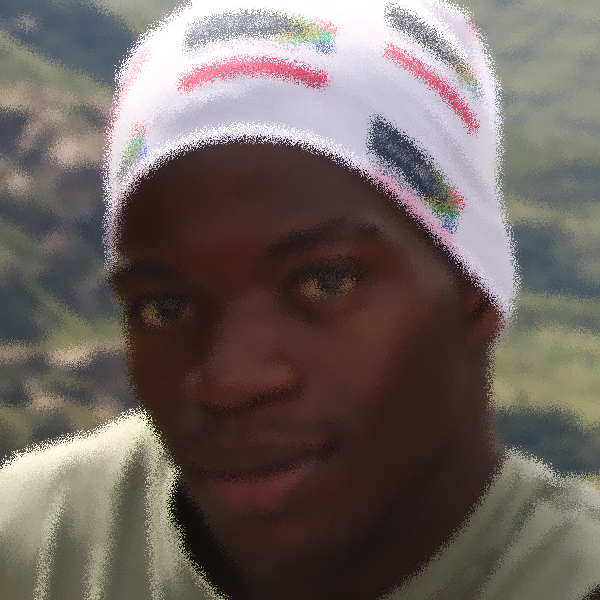
\includegraphics[width=0.48\linewidth]{../report/assets/diffuse_4.png}
  \end{columns}
\end{frame}

\begin{frame}{Crosshatch \& Hue Rotate Results}
  \begin{columns}
    \column{0.48\textwidth}
      \centering
      \textbf{Crosshatch}\\[4pt]
      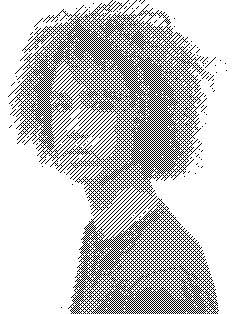
\includegraphics[width=0.48\linewidth]{../report/assets/cross_filtered_1.png}\hfill
      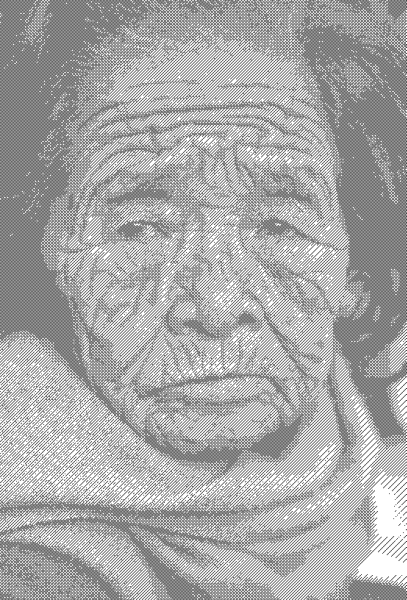
\includegraphics[width=0.48\linewidth]{../report/assets/cross_filtered_2.png}\\[2pt]
      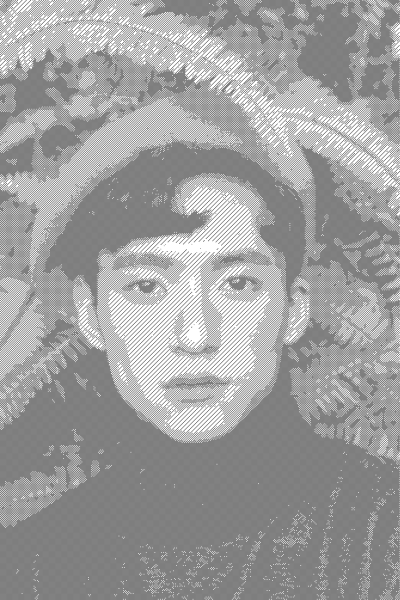
\includegraphics[width=0.48\linewidth]{../report/assets/cross_filtered_3.png}\hfill
      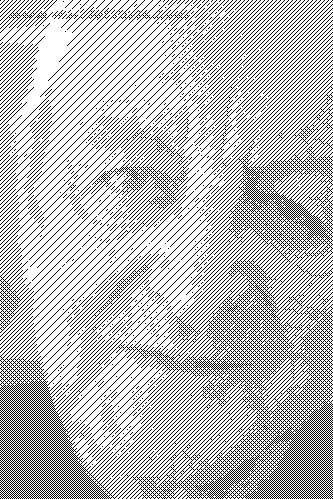
\includegraphics[width=0.48\linewidth]{../report/assets/cross_filtered_4.png}
    \column{0.48\textwidth}
      \centering
      \textbf{Hue Rotate}\\[4pt]
      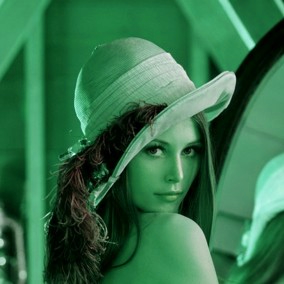
\includegraphics[width=0.48\linewidth]{../report/assets/hue_1.png}\hfill
      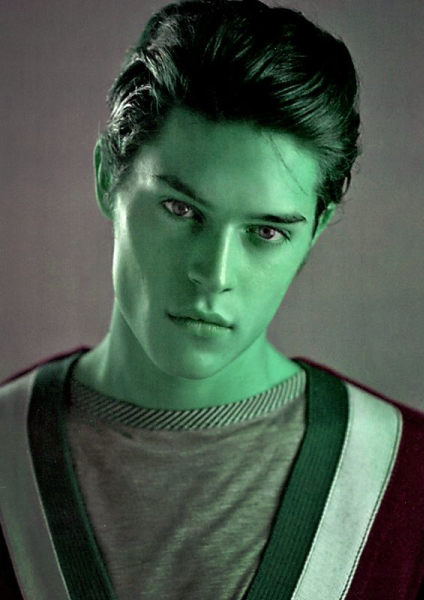
\includegraphics[width=0.48\linewidth]{../report/assets/hue_2.png}\\[2pt]
      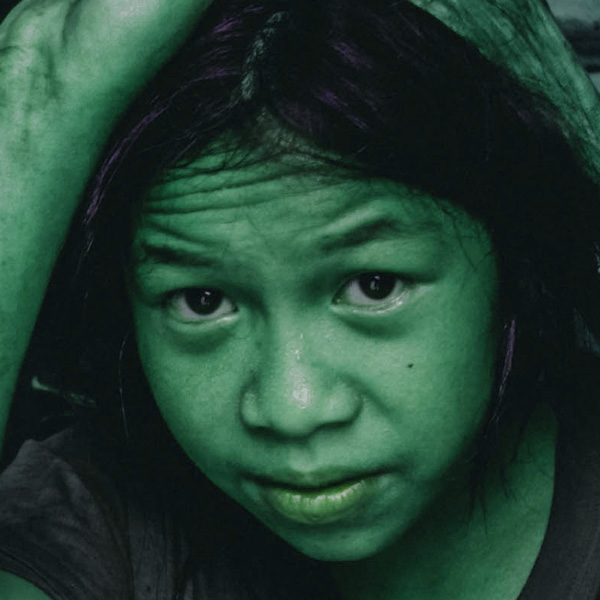
\includegraphics[width=0.48\linewidth]{../report/assets/hue_3.png}\hfill
      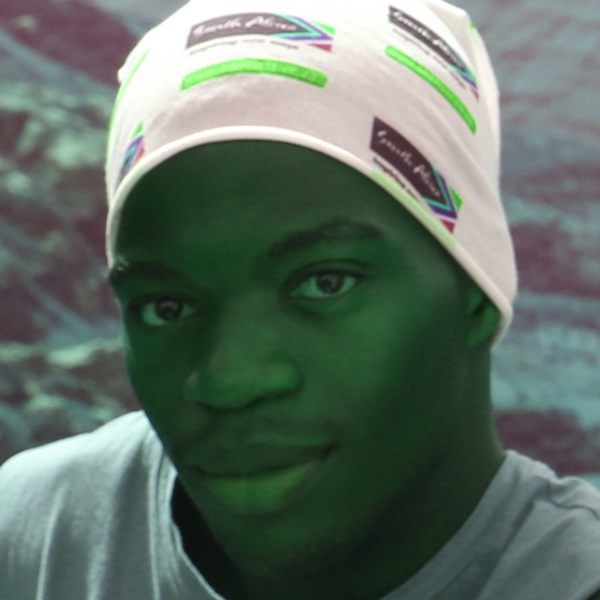
\includegraphics[width=0.48\linewidth]{../report/assets/hue_4.png}
  \end{columns}
\end{frame}

% =============================================================================
\section{Summary}
% =============================================================================

\begin{frame}{Summary}
  \begin{columns}[T]
    \column{0.55\textwidth}
      \begin{block}{What We Built}
        \begin{itemize}
          \item 12 manually implemented image filters
          \item Interactive OpenCV GUI with live preview
          \item Pixel-level C++ — no high-level filter APIs
          \item Modular architecture (one header per filter)
        \end{itemize}
      \end{block}
      \vspace{0.3cm}
      \begin{block}{Key Takeaways}
        \begin{itemize}
          \item All filters run in $O(W \times H)$ time
          \item LUTs improve per-pixel cost to array lookups
          \item YCrCb space prevents color drift in contrast ops
          \item Inverse mapping avoids holes in geometric warps
        \end{itemize}
      \end{block}
    \column{0.4\textwidth}
      \begin{block}{Filter Breakdown}
        \small
        \begin{tabular}{ll}
          \toprule
          \textbf{Author} & \textbf{Filters} \\
          \midrule
          Eyobed & Hist Eq, Lens Dist,\\
                 & Posterize, Vignette\\
          \midrule
          Adar   & Emboss, Dodge,\\
                 & Swirl, Bloom\\
          \midrule
          Deniz  & Threshold, Diffuse,\\
                 & Crosshatch, Hue Rot\\
          \bottomrule
        \end{tabular}
      \end{block}
  \end{columns}
\end{frame}

% ── Final Slide ──
\begin{frame}[plain]
  \begin{tikzpicture}[remember picture, overlay]
    \fill[bg] (current page.south west) rectangle (current page.north east);
  \end{tikzpicture}
  \vfill
  \centering
  {\color{accent}\Huge\textbf{Thank You}}\\[0.5cm]
  \textcolor{muted}{\rule{0.4\textwidth}{0.4pt}}\\[0.5cm]
  {\color{textlight}\large Questions?}\\[0.8cm]
  {\color{muted}
    Adar Otieno \quad Deniz Aksoy \quad Eyobed Awel Nuri\\[0.2cm]
    \small ZPOe 25/26 — Brno University of Technology
  }
  \vfill
\end{frame}

\end{document}
